\newpage
\begin{center}
\textbf{ГЛАВА 3}\\
\textbf{ДИФФУЗИЯ ОТ ТРОЙНОЙ ДО КРИТИЧЕСКОЙ ТОЧКИ}
\end{center}
\refstepcounter{chapter}


% \section*{}
\addcontentsline{toc}{chapter}{ГЛАВА 3. Диффузия от тройной до критической точки}


\section{Изучение диффузии методами молекулярной динамики}\label{C3_1}

Имея координаты всех частиц в системах, можно пронаблюдать за перемещение каждой частицей в отдельности, и оценить диффузию в данной системе.

На рисунке \ref{risTreck} изображены траектории частиц в  исходной исследуемой системе на примере потенциала Леннарда - Джонса. Для построения рисунка были взяты первые 10 кадров, используемые для статистики, описанной в разделе \ref{C2_2}, с шагом по времени между кадрами равными $0.5\tau$. Траектории раскрашены в зависимости от перемещения частицы за 10 кадров наблюдения. В данном случае наиболее оптимальным было взять цвет для максимального перемещения в $3\sigma$, где $\sigma$ - безразмерная единица измерения длинны в моделировании, равная единице. 

\begin{figure}[htbp!]
\begin{center}
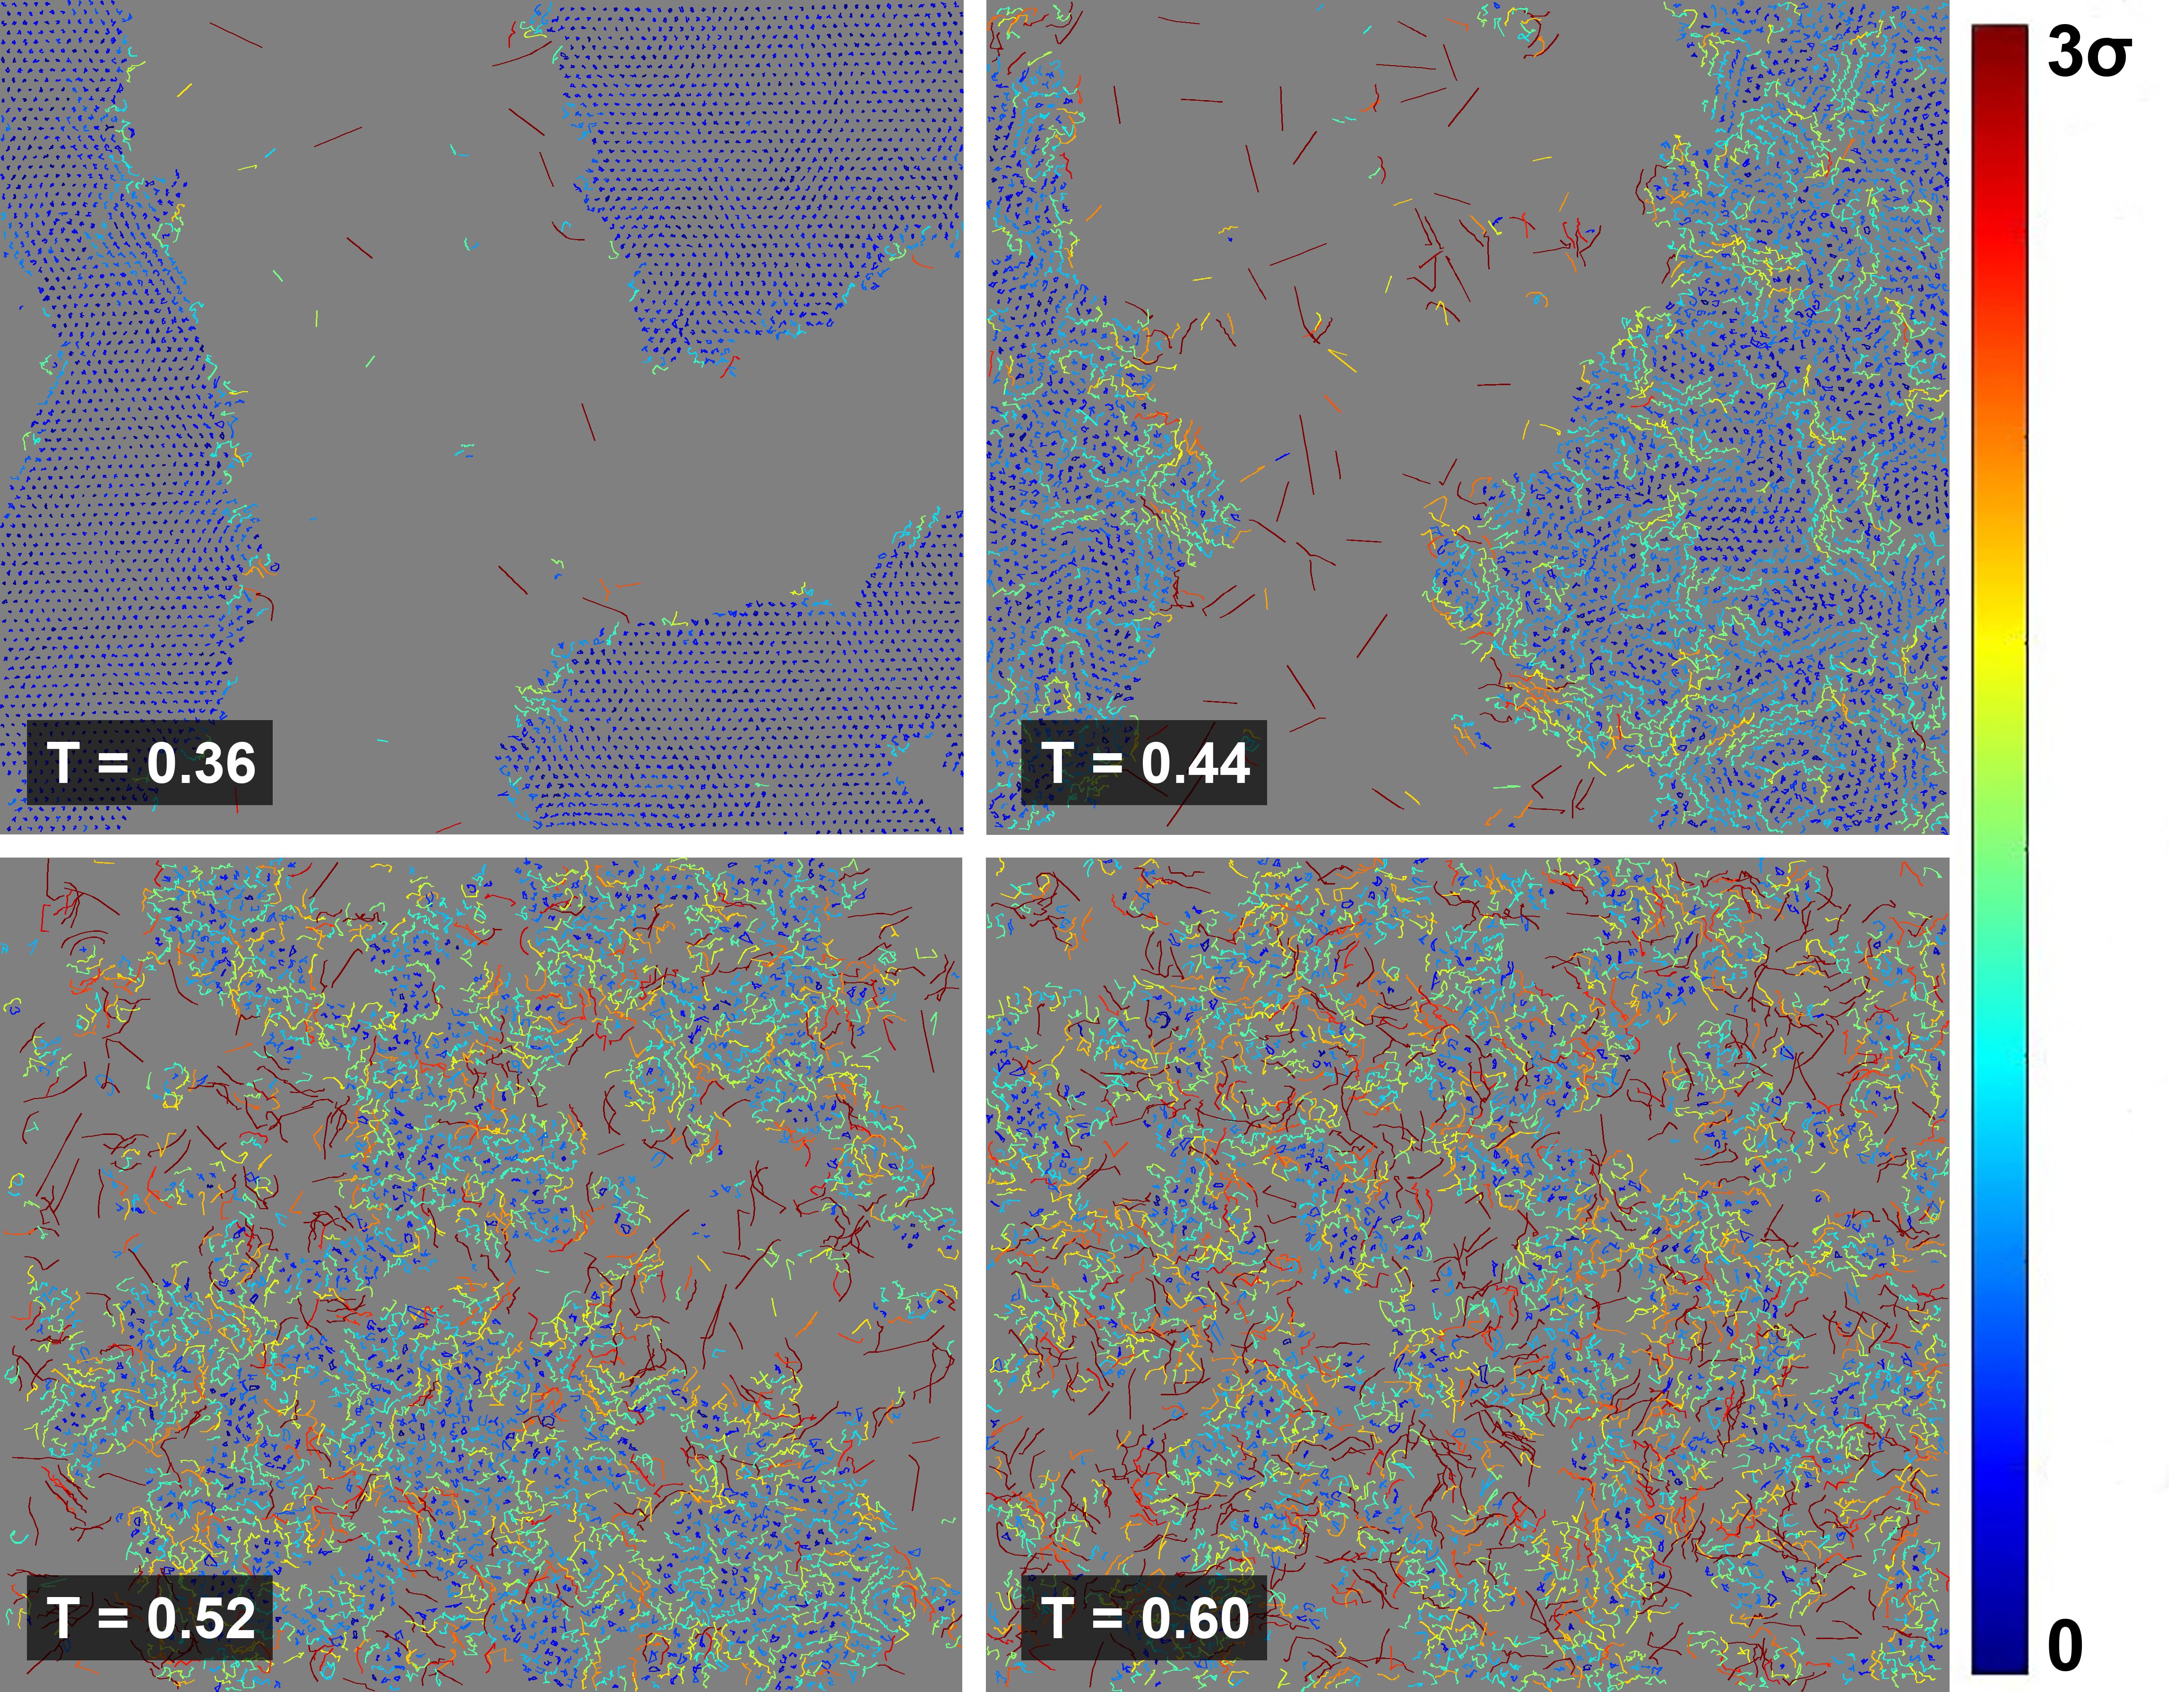
\includegraphics[width=0.7\textwidth]{Diffusion}
\caption{Смещение частиц от начального положения за 10 кадров моделирования. Цветом показана величина смещения в $\sigma$ (единица измерения длинны).}
\label{risTreck}
\end{center}
\end{figure}

Зная смещения всех частиц от их изначального положения в системе, с $t = 0$, можно расчитать среднеквадратичное смещение частиц в системе с помощью уравнения:
\begin{equation}
    \sigma^2(t) = \sum\limits_{\alpha = 1}^{N(t)} (r_{\alpha}(t) - r_{\alpha}(0))^2 / N(t),
    \label{eqRMS}
\end{equation}
где $\sigma^2(t)$ - среднеквадратичное смещение частиц; $N(t)$ - количество частиц в исследуемой подсистеме; $r_{\alpha}(t)$ - положение частицы в момент времени $t$; $r_{\alpha}(0)$ - положение частицы в начальный момент времени $t = 0$.

\begin{figure}[h]
\begin{center}
\begin{minipage}[h]{0.45\linewidth}
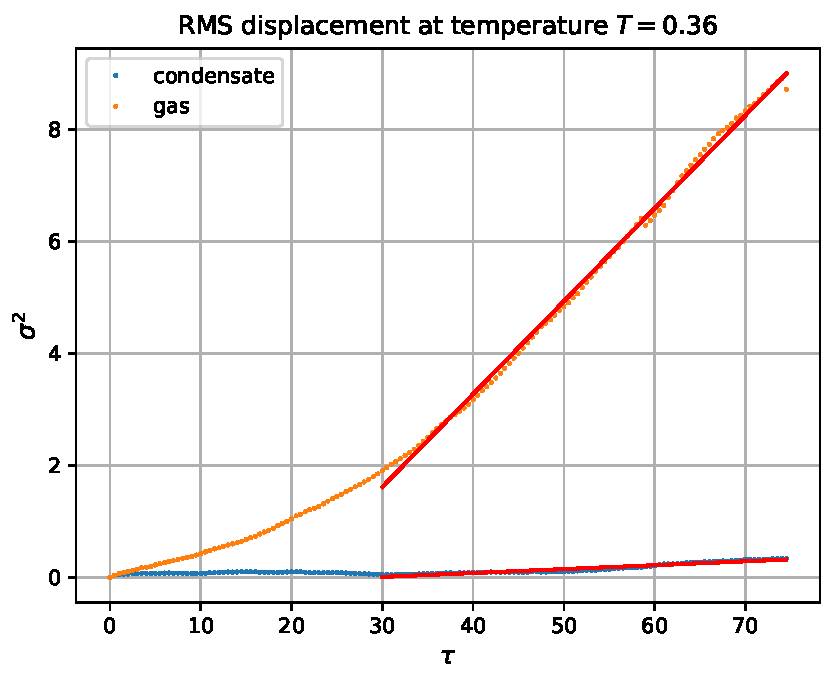
\includegraphics[width=\textwidth, keepaspectratio]{diffusion_fit_0.36}
\end{minipage}
%\hfill
\begin{minipage}[h]{0.45\linewidth}
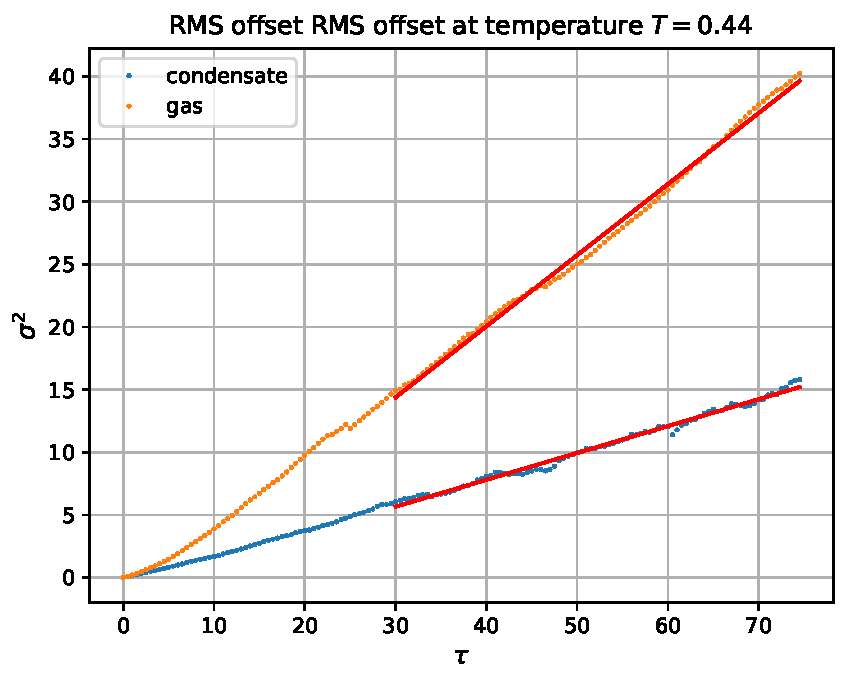
\includegraphics[width=\textwidth, keepaspectratio]{diffusion_fit_0.44}
\end{minipage}

%\vfill

\begin{minipage}[h]{0.45\linewidth}
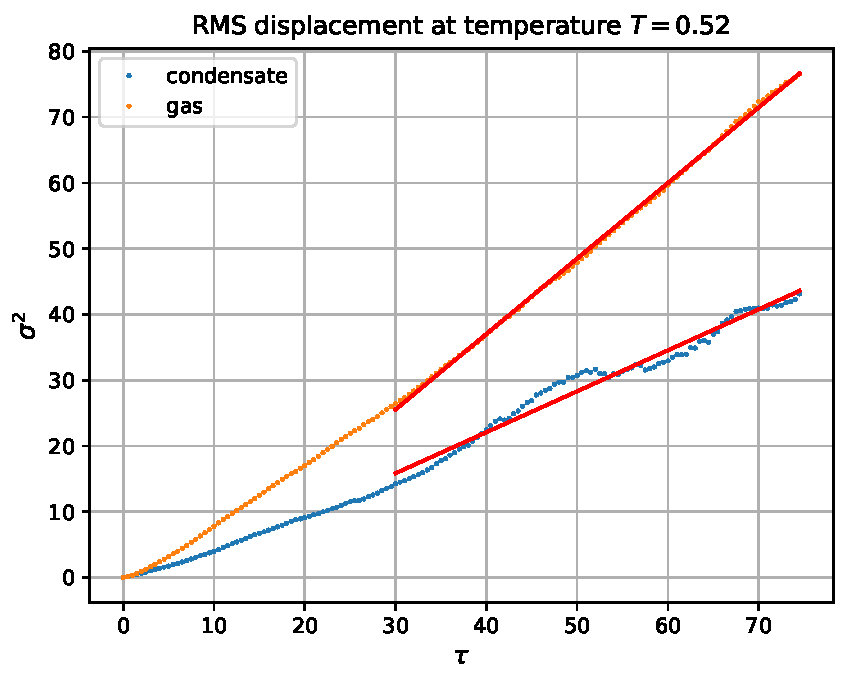
\includegraphics[width=\textwidth, keepaspectratio]{diffusion_fit_0.52}
\end{minipage}
%\hfill
\begin{minipage}[h]{0.45\linewidth}
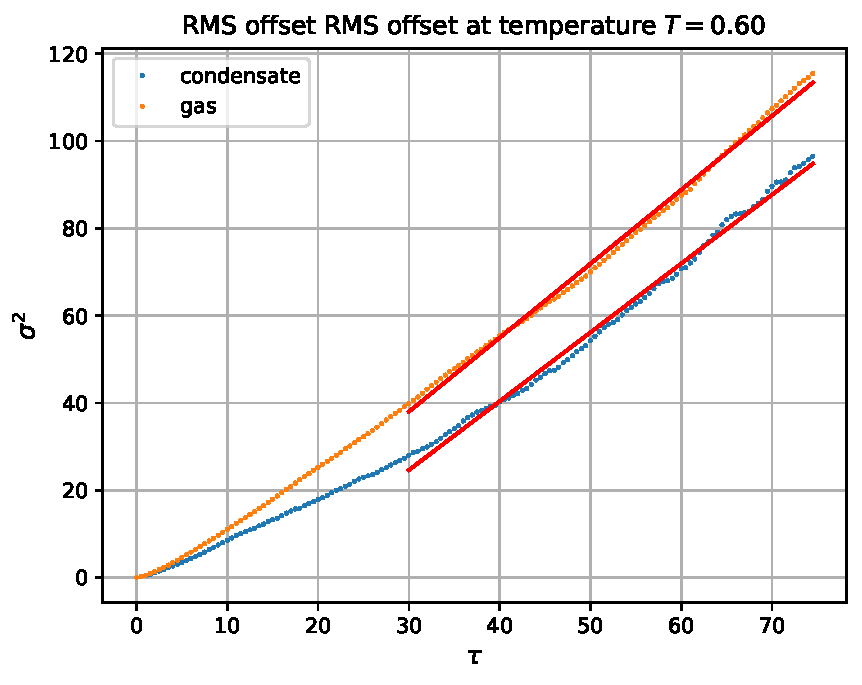
\includegraphics[width=\textwidth, keepaspectratio]{diffusion_fit_0.60}
\end{minipage}
\caption{Временная зависимость среднеквадратичного смещения частиц для различных температур на примере потенциала Леннарда-Джонса. Синим цветом обозначено среднеквадратичное смещение конденсированных частиц,  а оранжевым - всех частиц в исследуемой системе.}
\label{risRMS}
\end{center}
\end{figure}

График зависимости среднеквадратичного смещения для подсистем конденсированных частиц и всех (все частицы в системе, включая газовые и конденсат) от безразмерного времени для различных температур изображен на рисунке \ref{risRMS}.

Так как для двумерной системы верно равенство $\sigma^2(t) = 4Dt$, то коэффициент диффузии выражается следующей формулой:
\begin{equation}
    D = \frac{\sigma^2(t)}{4t},
    \label{eqD}
\end{equation}
где $D$ - коэффициент диффузии в веществе.

Его можно получить путем аппроксимации среднеквадратичного смещения функцией $\sigma^2(t) = 4Dt + a$, где $а$ - подгоночный коэффициент. Аппроксимация производится начиная не с 0 по времени, а с некоторого значения, когда функция становится линейной. Данный эффект хорошо наблюдается при $T = 0.36$ на рисунке \ref{risRMS}. Наблюдения показывают, что для данных экспериментов достаточно использовать последние $60\%$ точек, для правильной аппроксимации.  

\begin{figure}[h]
\begin{center}
\begin{minipage}[h]{0.45\linewidth}
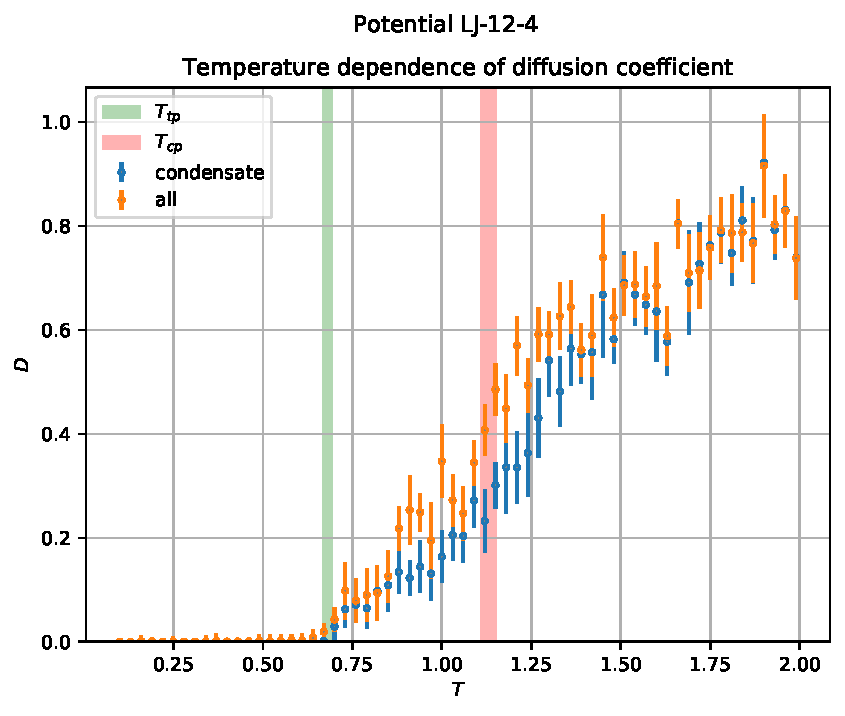
\includegraphics[width=\textwidth, keepaspectratio]{plot_diffusion_Potential LJ-12-4_1}
\end{minipage}
\begin{minipage}[h]{0.45\linewidth}
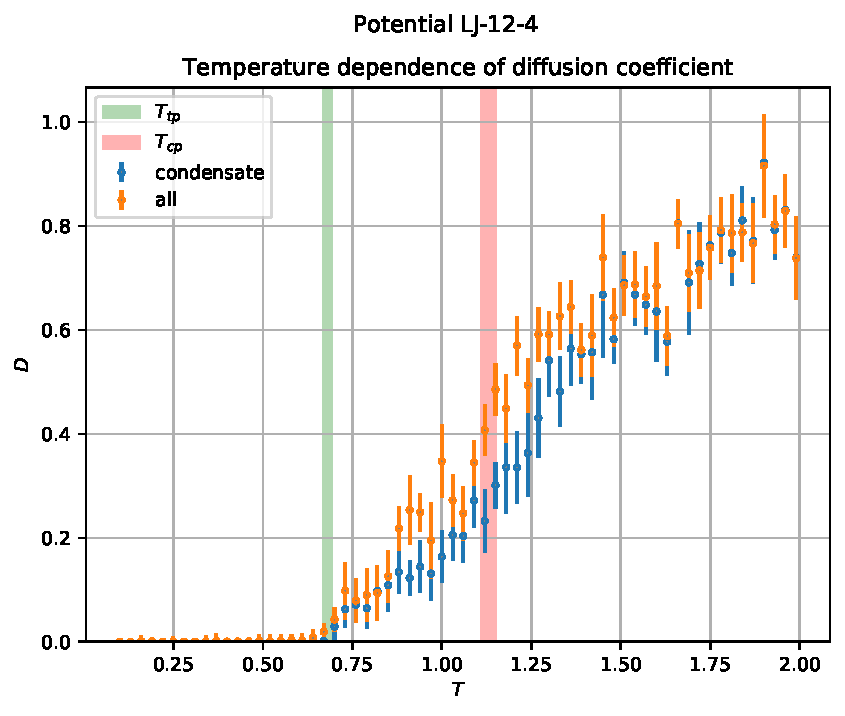
\includegraphics[width=\textwidth, keepaspectratio]{plot_diffusion_Potential LJ-12-4_1}
\end{minipage}
\begin{minipage}[h]{0.45\linewidth}
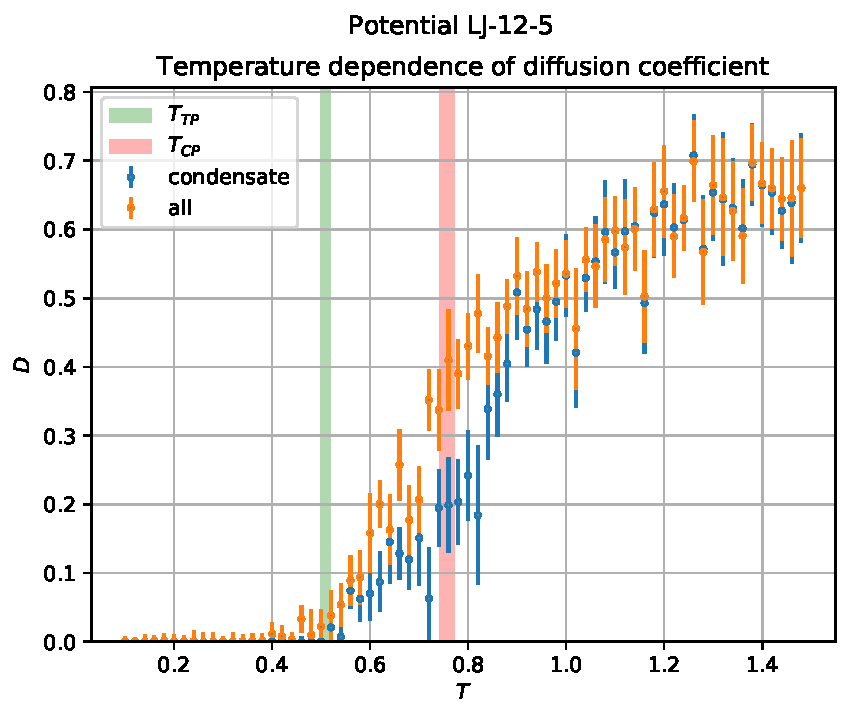
\includegraphics[width=\textwidth, keepaspectratio]{plot_diffusion_Potential LJ-12-5_1}
\end{minipage}
\begin{minipage}[h]{0.45\linewidth}
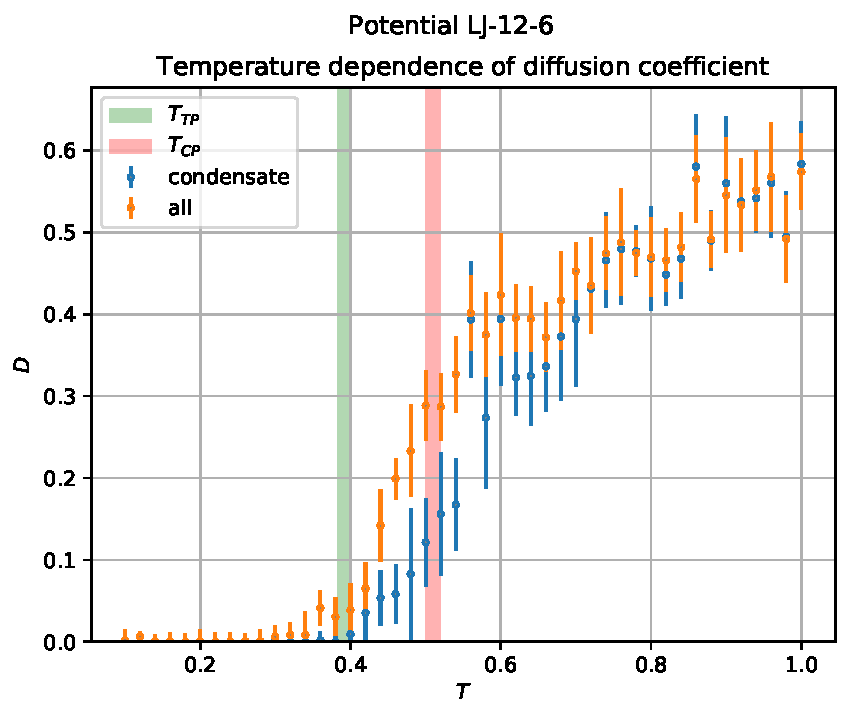
\includegraphics[width=\textwidth, keepaspectratio]{plot_diffusion_Potential LJ-12-6_1}
\end{minipage}
\caption{Температурная зависимость коэффициента диффузии для различных потенциалов взаимодействия. Не доделана!}
\label{risD}
\end{center}
\end{figure}

Проводя данные вычисления для различных температур, можно установить температурную зависимость коэффициента диффузии для различных потенциалов взаимодействия, изображенную на рисунке \ref{risD}.

\begin{figure}[htbp!]
\begin{center}
\begin{minipage}[h]{0.45\linewidth}
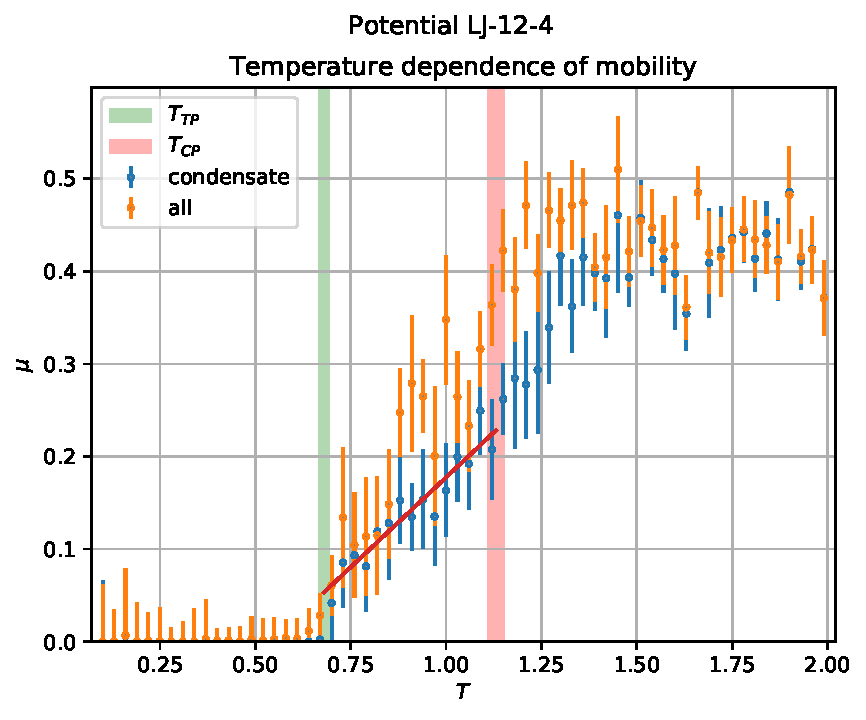
\includegraphics[width=\textwidth, keepaspectratio]{plot_mobility_Potential LJ-12-4_1}
\end{minipage}
%\hfill
\begin{minipage}[h]{0.45\linewidth}
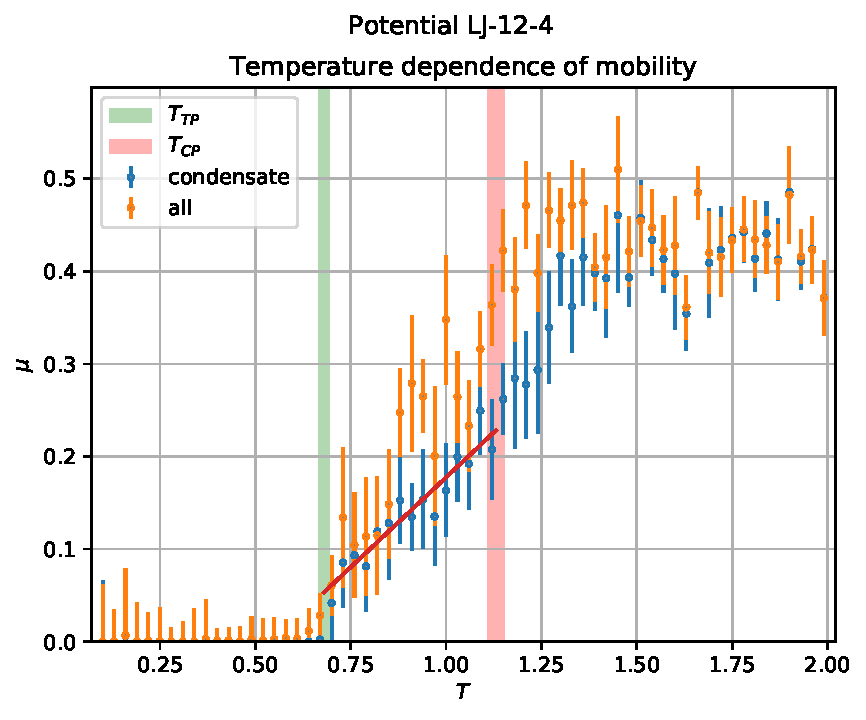
\includegraphics[width=\textwidth, keepaspectratio]{plot_mobility_Potential LJ-12-4_1}
\end{minipage}
\begin{minipage}[h]{0.45\linewidth}
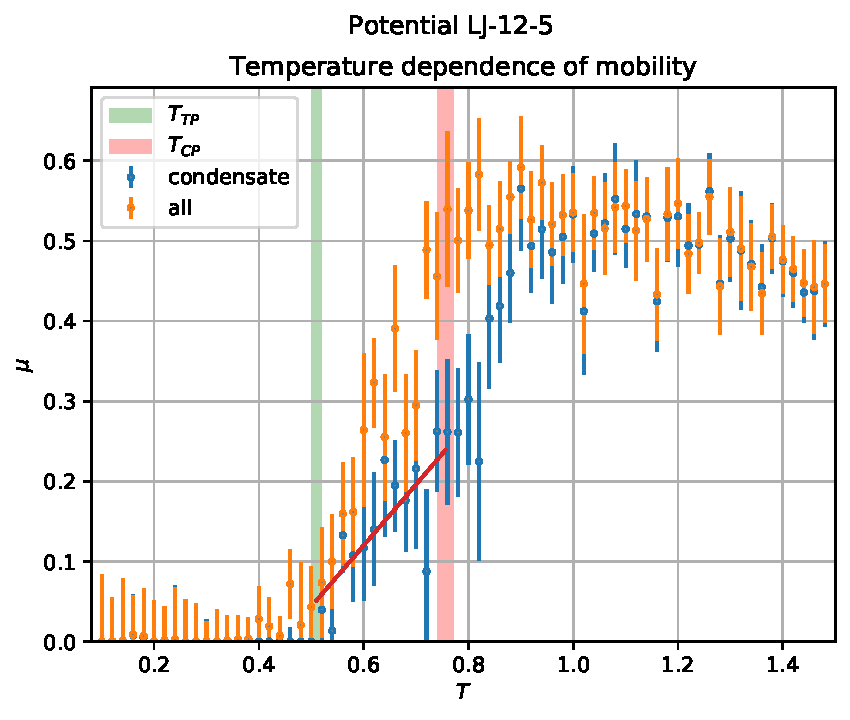
\includegraphics[width=\textwidth, keepaspectratio]{plot_mobility_Potential LJ-12-5_1}
\end{minipage}
%\hfill
\begin{minipage}[h]{0.45\linewidth}
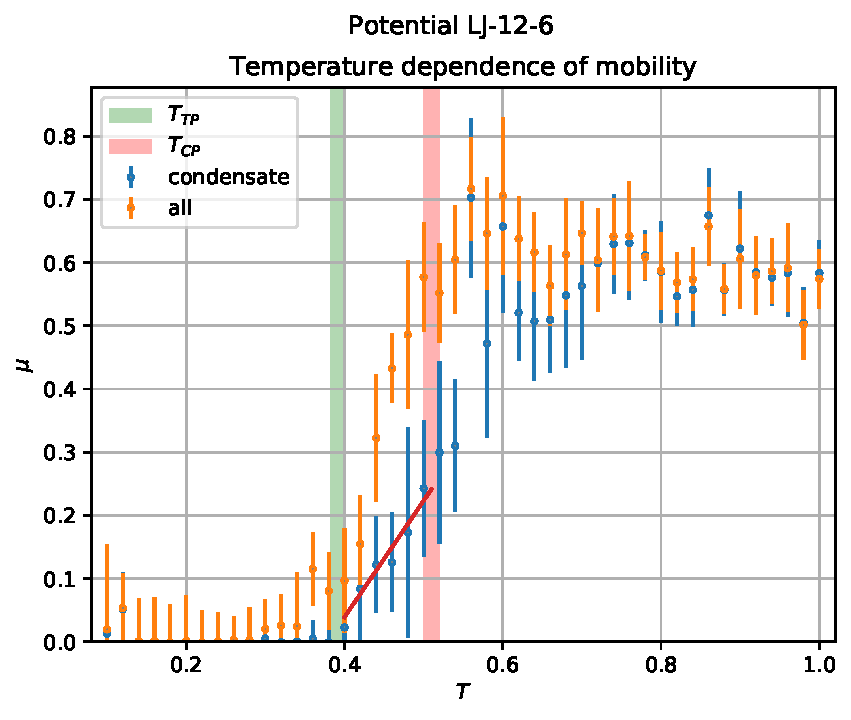
\includegraphics[width=\textwidth, keepaspectratio]{plot_mobility_Potential LJ-12-6_1}
\end{minipage}
\caption{Температурная зависимость мобильности для различных потенциалов взаимодействия. Не доделана!}
\label{ris18}
\end{center}
\end{figure}

Текст

Текст

\begin{figure}[htbp!]
\begin{center}
\begin{minipage}[h]{0.45\linewidth}
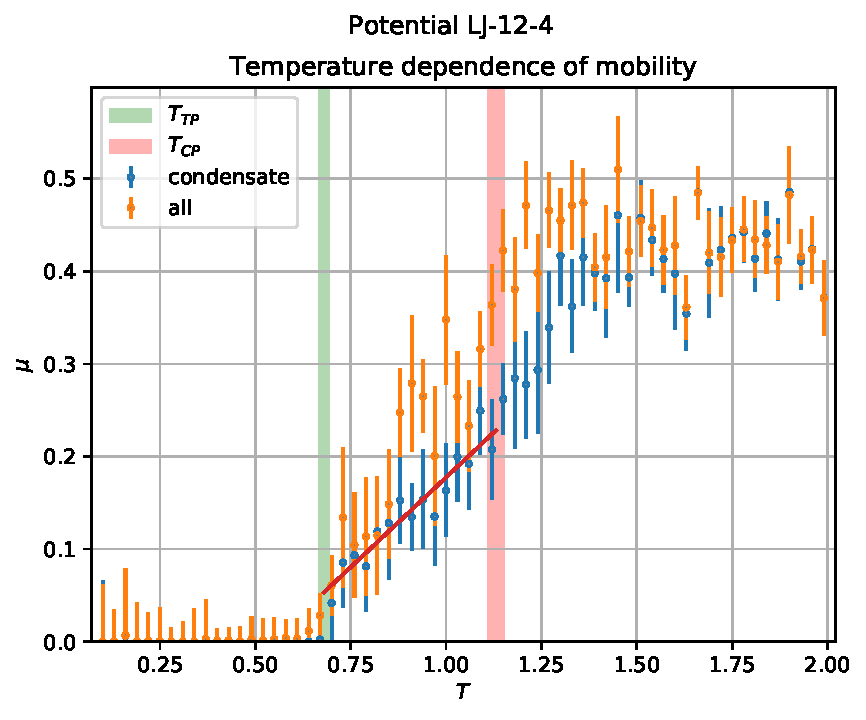
\includegraphics[width=\textwidth, keepaspectratio]{plot_mobility_Potential LJ-12-4_1}
\end{minipage}
%\hfill
\begin{minipage}[h]{0.45\linewidth}
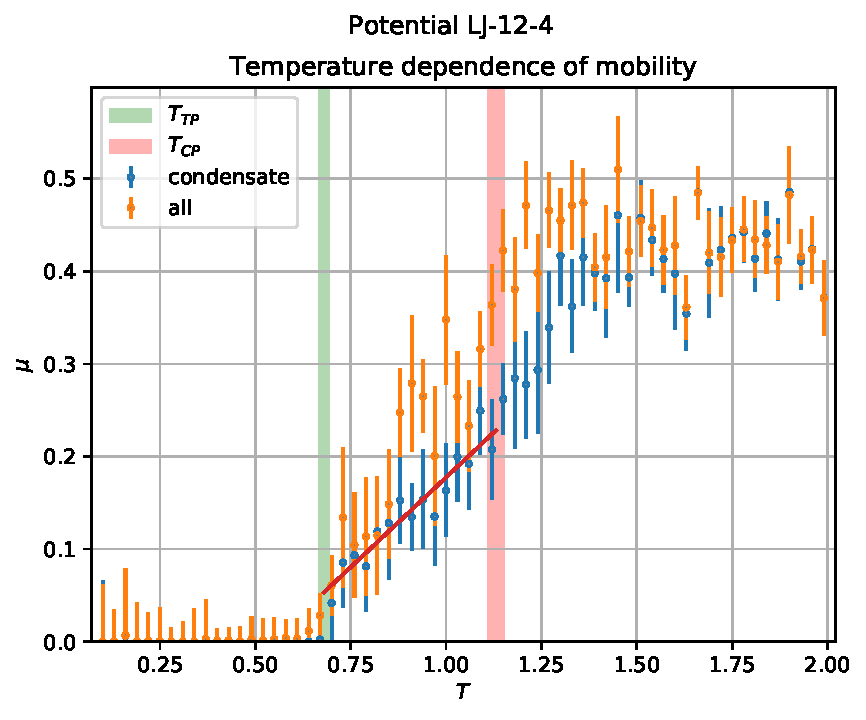
\includegraphics[width=\textwidth, keepaspectratio]{plot_mobility_Potential LJ-12-4_1}
\end{minipage}

%\vfill

\begin{minipage}[h]{0.45\linewidth}
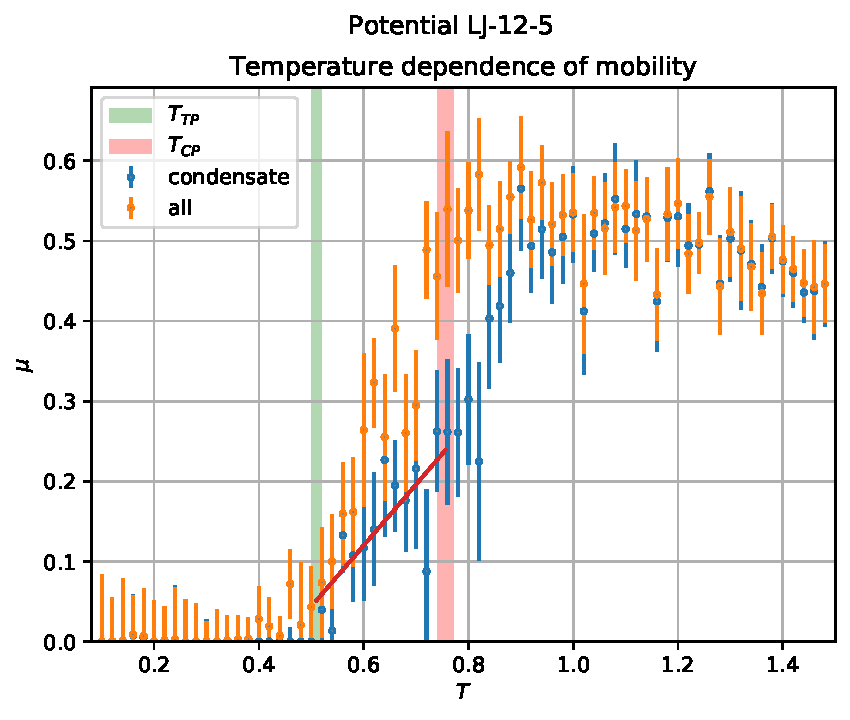
\includegraphics[width=\textwidth, keepaspectratio]{plot_mobility_Potential LJ-12-5_1}
\end{minipage}
%\hfill
\begin{minipage}[h]{0.45\linewidth}
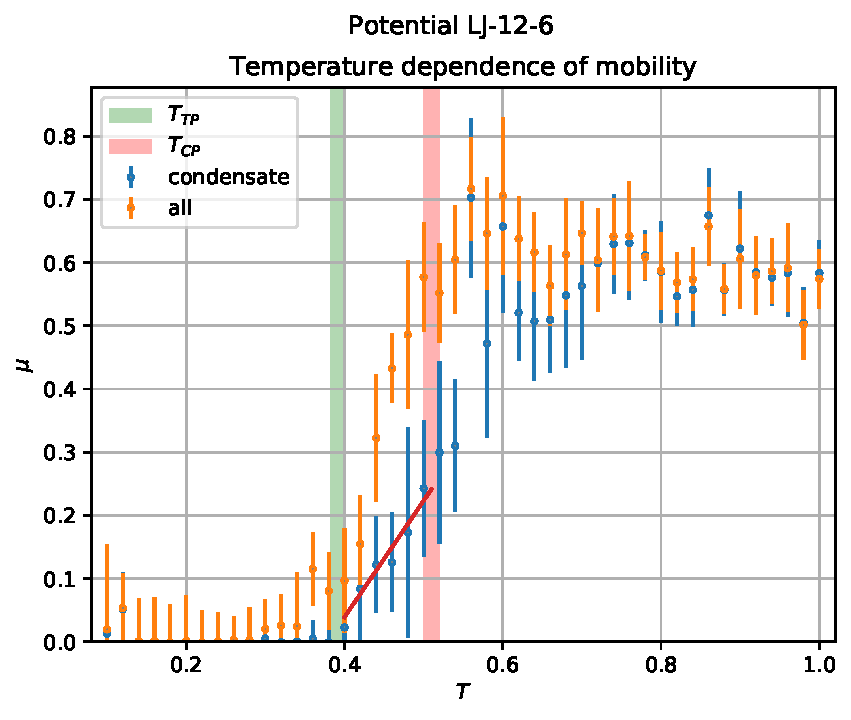
\includegraphics[width=\textwidth, keepaspectratio]{plot_mobility_Potential LJ-12-6_1}
\end{minipage}
\caption{Температурная зависимость мобильности для различных потенциалов взаимодействия. Не доделана!}
\label{ris19}
\end{center}
\end{figure}

Текст

\section{Связь термодинамических параметров, и параметров переноса вещества}\label{C3_2}

Текст

Текст

\begin{figure}[htbp!]
\begin{center}
\begin{minipage}[h]{0.45\linewidth}
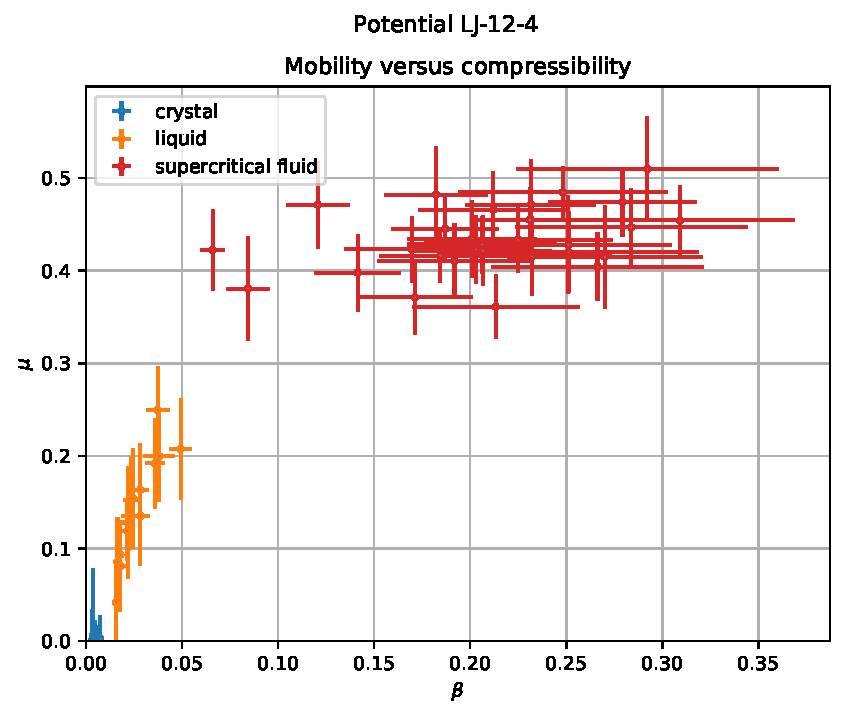
\includegraphics[width=\textwidth, keepaspectratio]{plot_compress_mobility_Potential LJ-12-4_1}
\end{minipage}
%\hfill
\begin{minipage}[h]{0.45\linewidth}
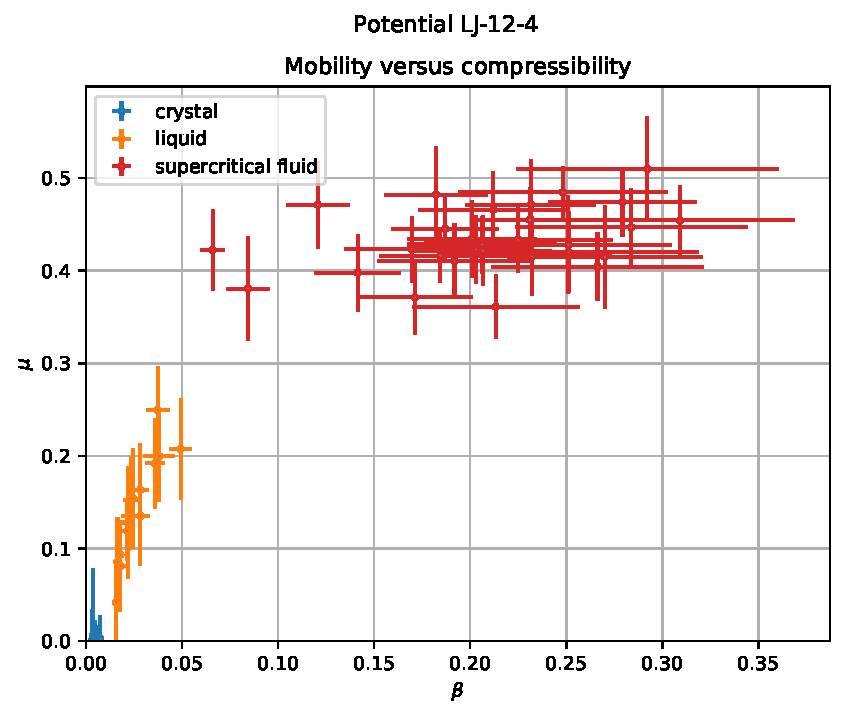
\includegraphics[width=\textwidth, keepaspectratio]{plot_compress_mobility_Potential LJ-12-4_1}
\end{minipage}

%\vfill

\begin{minipage}[h]{0.45\linewidth}
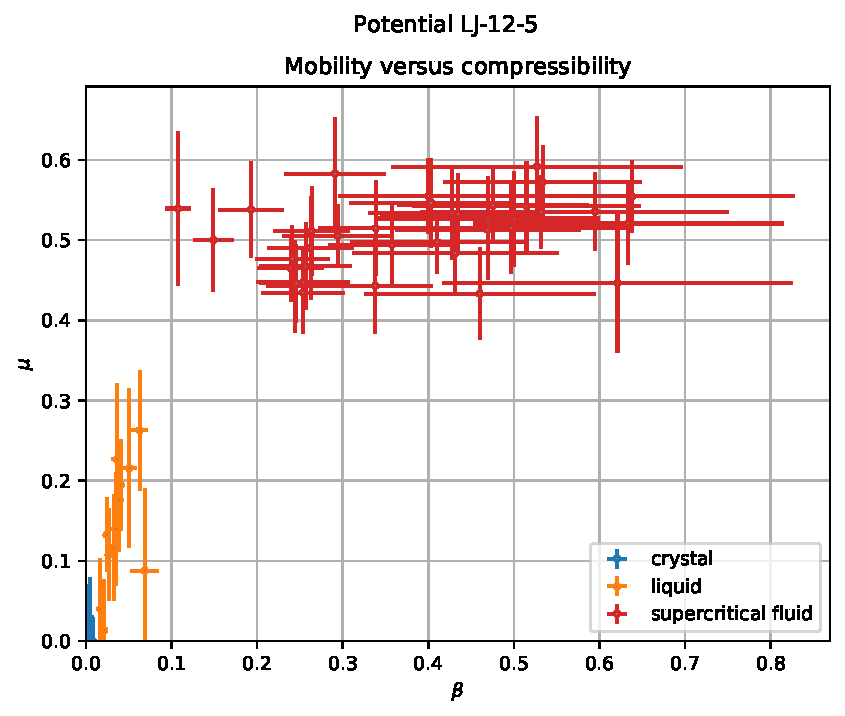
\includegraphics[width=\textwidth, keepaspectratio]{plot_compress_mobility_Potential LJ-12-5_1}
\end{minipage}
%\hfill
\begin{minipage}[h]{0.45\linewidth}
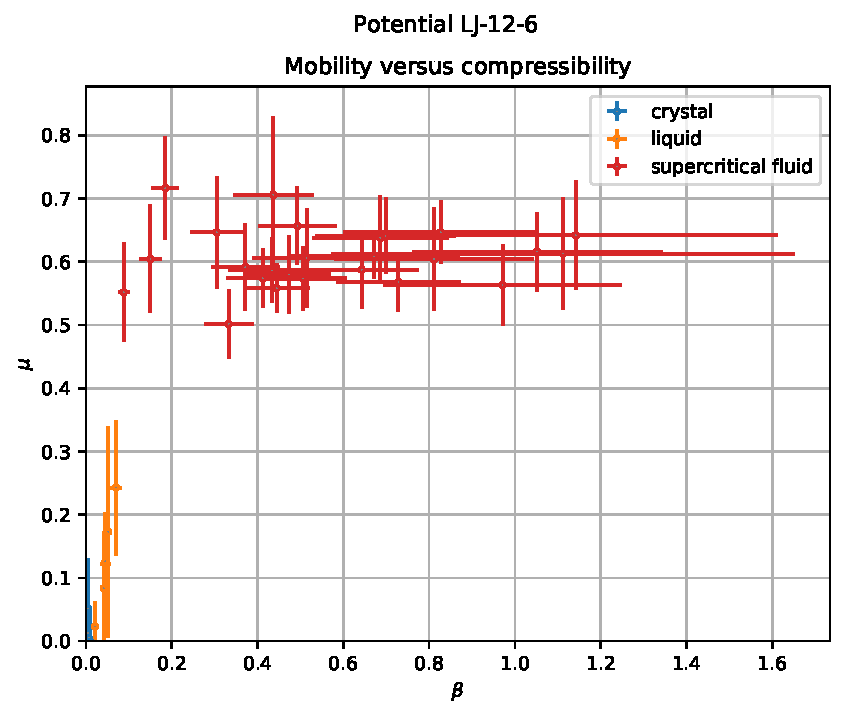
\includegraphics[width=\textwidth, keepaspectratio]{plot_compress_mobility_Potential LJ-12-6_1}
\end{minipage}
\caption{Зависимость мобильности от сжимаемости. Не доделана!}
\label{ris20}
\end{center}
\end{figure}

Текст

Текст

\begin{figure}[htbp!]
\begin{center}
\begin{minipage}[h]{0.45\linewidth}
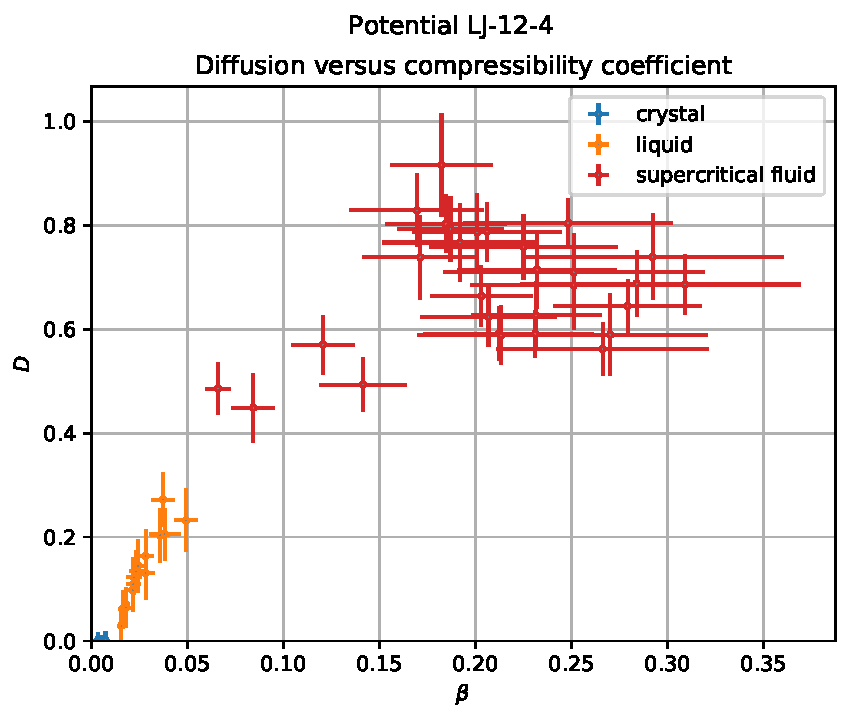
\includegraphics[width=\textwidth, keepaspectratio]{plot_diffusion_compress_Potential LJ-12-4_1}
\end{minipage}
%\hfill
\begin{minipage}[h]{0.45\linewidth}
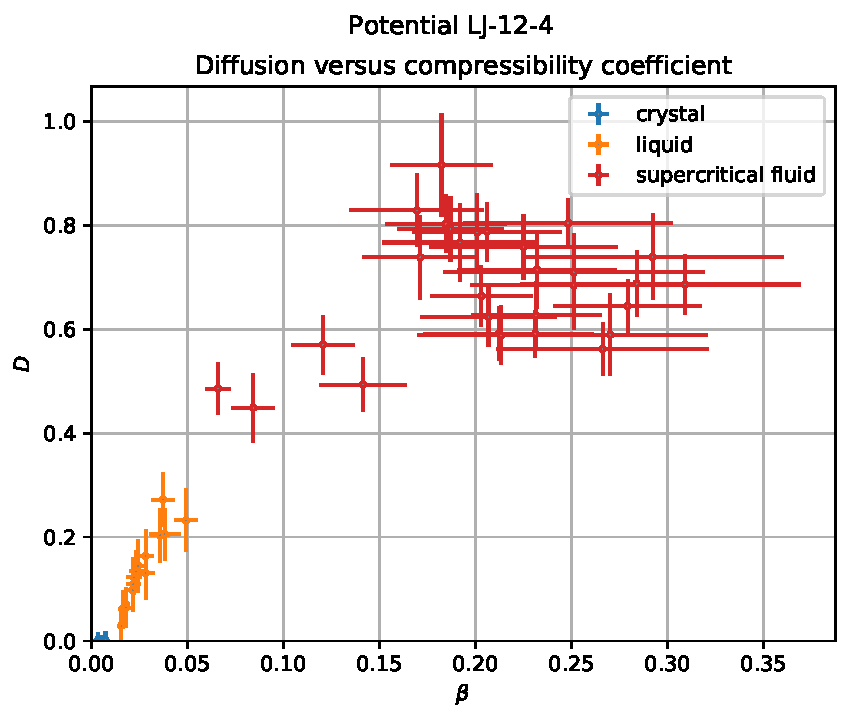
\includegraphics[width=\textwidth, keepaspectratio]{plot_diffusion_compress_Potential LJ-12-4_1}
\end{minipage}

%\vfill

\begin{minipage}[h]{0.45\linewidth}
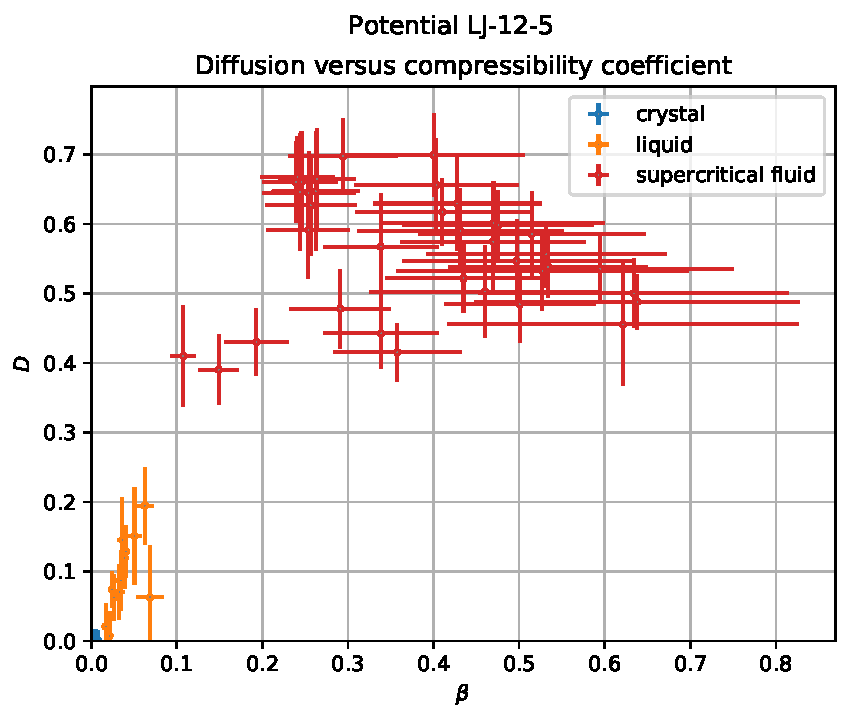
\includegraphics[width=\textwidth, keepaspectratio]{plot_diffusion_compress_Potential LJ-12-5_1}
\end{minipage}
%\hfill
\begin{minipage}[h]{0.45\linewidth}
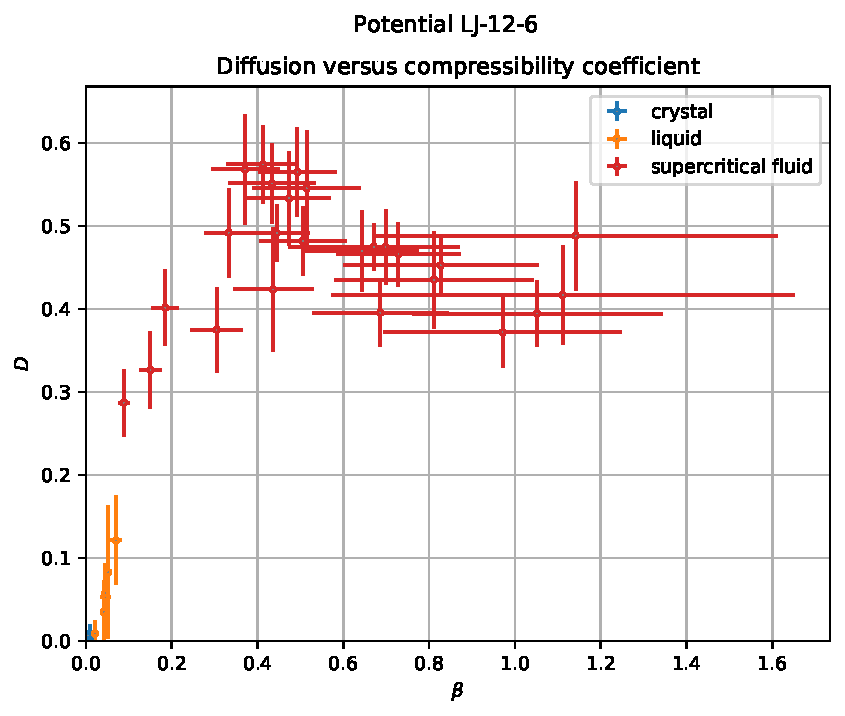
\includegraphics[width=\textwidth, keepaspectratio]{plot_diffusion_compress_Potential LJ-12-6_1}
\end{minipage}
\caption{Зависимость мобильности от сжимаемости. Не доделана!}
\label{ris21}
\end{center}
\end{figure}

Текст

Текст

\begin{figure}[htbp!]
\begin{center}
\begin{minipage}[h]{0.45\linewidth}
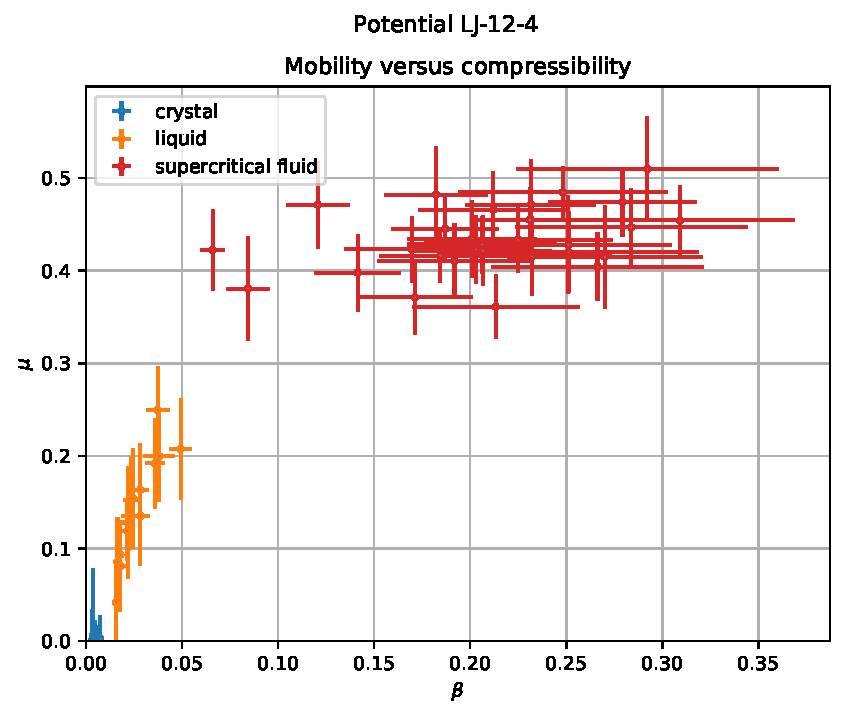
\includegraphics[width=\textwidth, keepaspectratio]{plot_compress_mobility_Potential LJ-12-4_1}
\end{minipage}
%\hfill
\begin{minipage}[h]{0.45\linewidth}
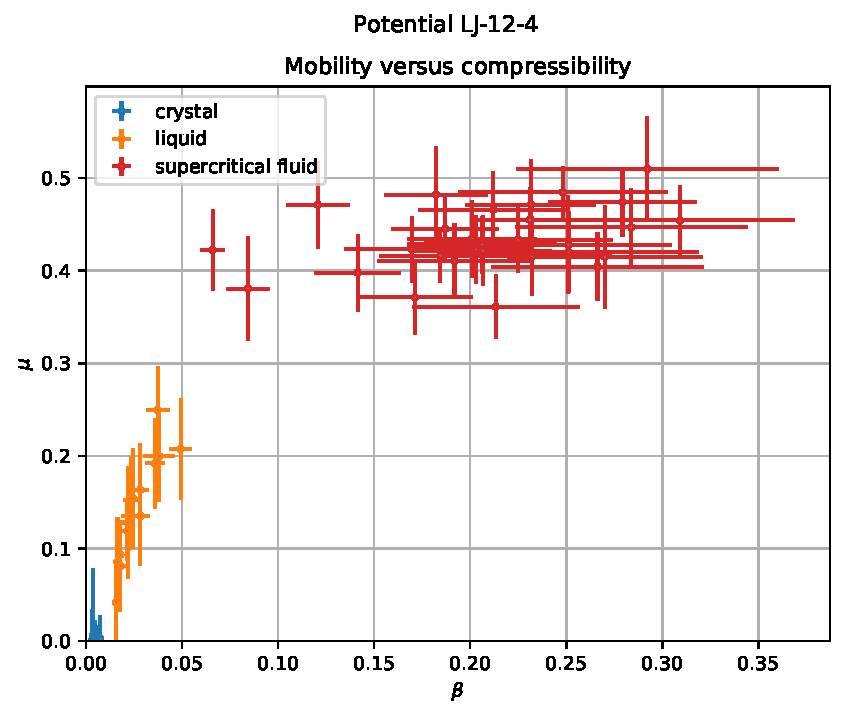
\includegraphics[width=\textwidth, keepaspectratio]{plot_compress_mobility_Potential LJ-12-4_1}
\end{minipage}

%\vfill

\begin{minipage}[h]{0.45\linewidth}
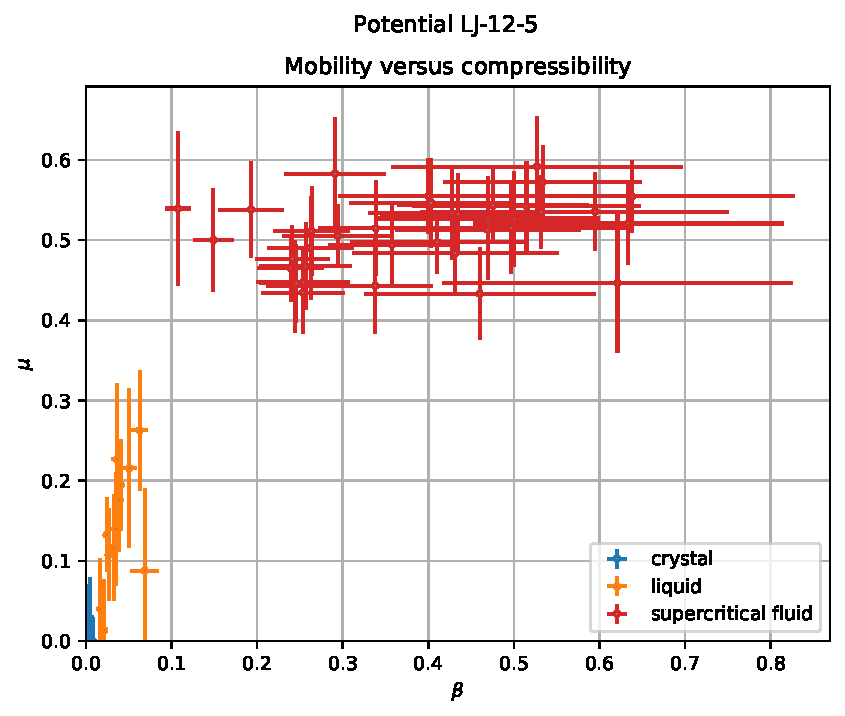
\includegraphics[width=\textwidth, keepaspectratio]{plot_compress_mobility_Potential LJ-12-5_1}
\end{minipage}
%\hfill
\begin{minipage}[h]{0.45\linewidth}
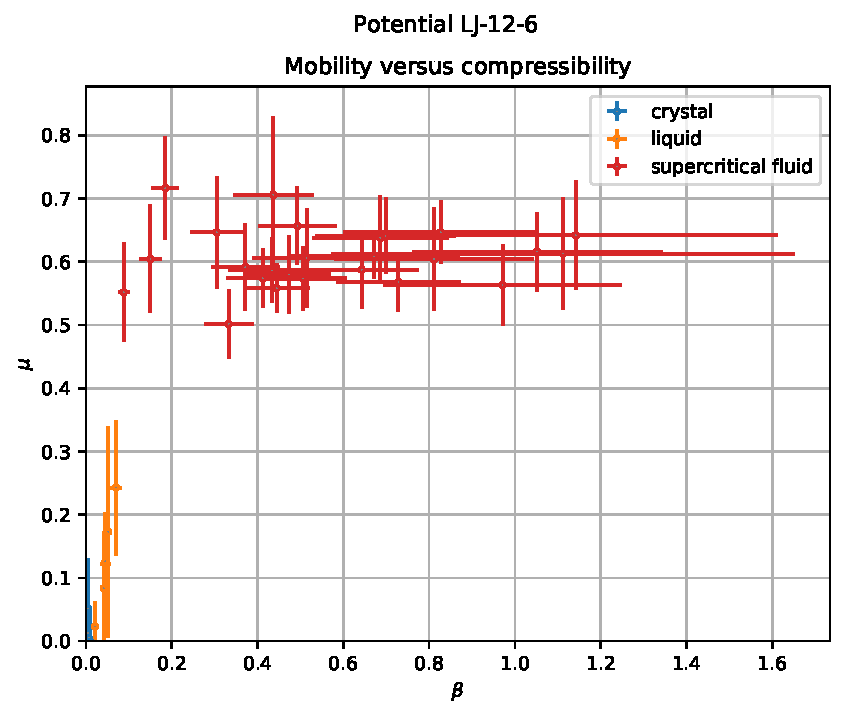
\includegraphics[width=\textwidth, keepaspectratio]{plot_compress_mobility_Potential LJ-12-6_1}
\end{minipage}
\caption{Зависимость мобильности от сжимаемости. Не доделана!}
\label{ris22}
\end{center}
\end{figure}

Текст

Текст

\begin{figure}[htbp!]
\begin{center}
\begin{minipage}[h]{0.45\linewidth}
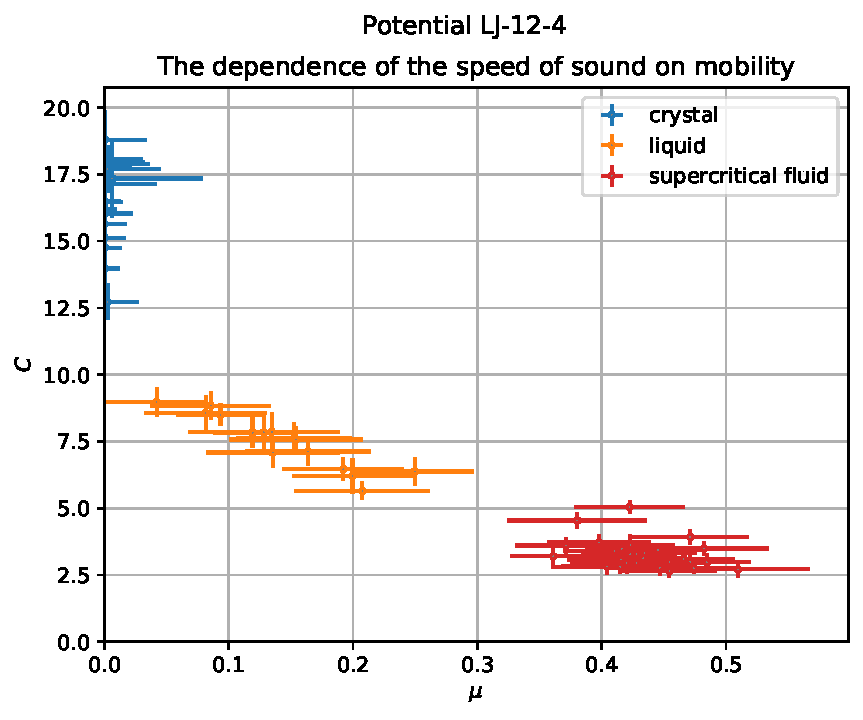
\includegraphics[width=\textwidth, keepaspectratio]{sound_speed_mobility_Potential LJ-12-4_1}
\end{minipage}
%\hfill
\begin{minipage}[h]{0.45\linewidth}
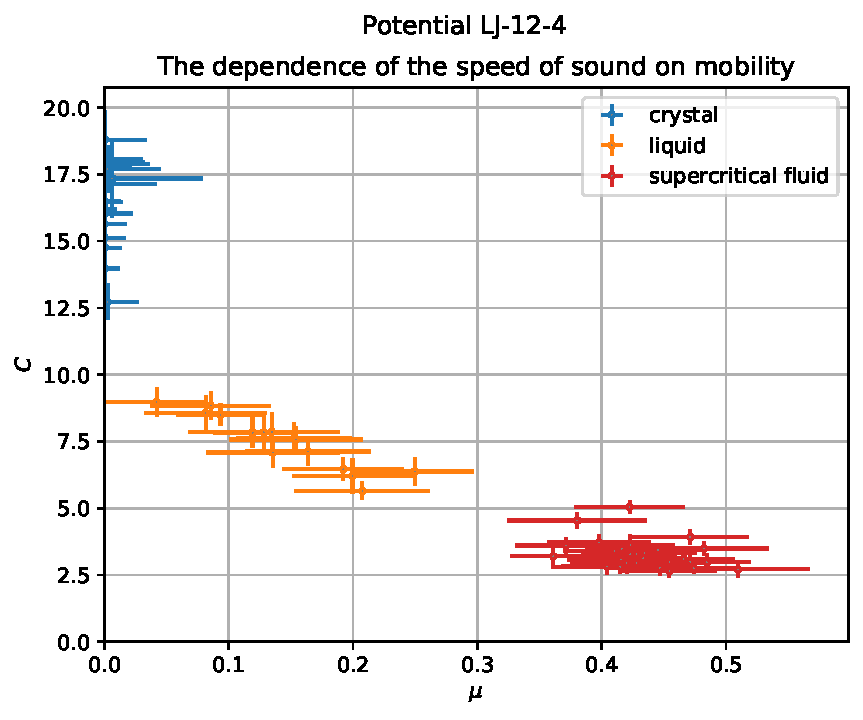
\includegraphics[width=\textwidth, keepaspectratio]{sound_speed_mobility_Potential LJ-12-4_1}
\end{minipage}

%\vfill

\begin{minipage}[h]{0.45\linewidth}
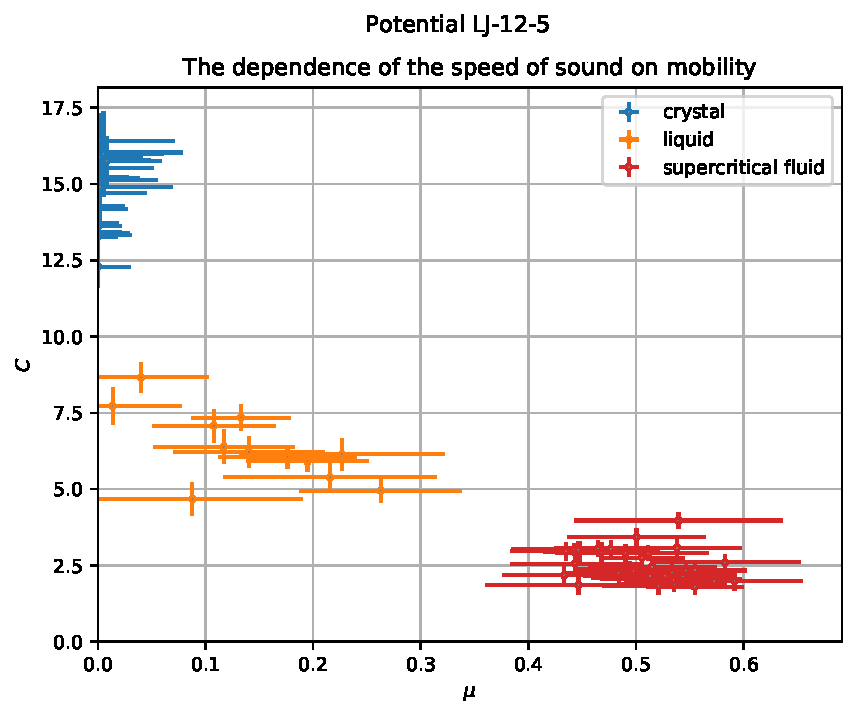
\includegraphics[width=\textwidth, keepaspectratio]{sound_speed_mobility_Potential LJ-12-5_1}
\end{minipage}
%\hfill
\begin{minipage}[h]{0.45\linewidth}
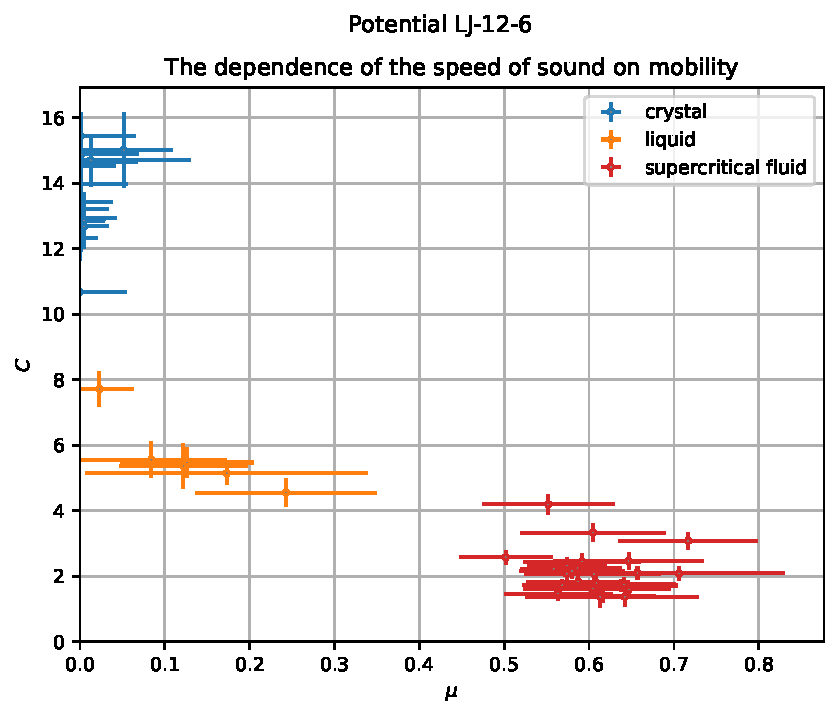
\includegraphics[width=\textwidth, keepaspectratio]{sound_speed_mobility_Potential LJ-12-6_1}
\end{minipage}
\caption{Зависимость мобильности от сжимаемости. Не доделана!}
\label{ris23}
\end{center}
\end{figure}

Текст

\section{Выводы главы}\label{C3_3}

Вывод